\begin{frame}
	\frametitle{Procedimento 03}
	\framesubtitle{Descrição}
	\only<1>{
		\begin{itemize}
			\item 300 testes aleatórios em cada caso.
			\item EER = equilibrio entre as taxas de falsos positivos e de falsos negativos.
			\item Em alguns casos o cálculo do EER necessitou mais iterações.
			\item 10\%, 20\%, 30\%, 40\% e 50\% da base de sinais reservados para treinamento.
		\end{itemize}
	}	
\end{frame}

\begin{frame}
	\frametitle{Procedimento 03}
	\framesubtitle{Tabela de resultados}
	\begin{table}[H]
	\newcommand{\mc}[3]{\multicolumn{#1}{#2}{#3}}
	\definecolor{tcA}{rgb}{0.65098,0.65098,0.65098}
	\definecolor{tcB}{rgb}{0.447059,0.74902,0.266667}
	\begin{center}
		\caption{Resultados da abordagem com SVM}
		\begin{tabular}{|p{0.15\linewidth}|p{0.11\linewidth}|p{0.11\linewidth}|p{0.11\linewidth}|p{0.14\linewidth}|p{0.14\linewidth}|}\hline
			% use packages: color,colortbl
			\rowcolor{tcA}
			\centering\textbf{$M$} & \centering\textbf{Acurácia mínima} & \centering\textbf{Acurácia máxima} & \centering\textbf{Média das acurácias} & \centering\textbf{Desvio padrão da acurácia} & \begin{center}\textbf{EER}\end{center}\\\hline
			
			\rowcolor{tcB}
			% Loads data from tables/results/paraconsistentPlane/distParacomFrom10.csv
			\csvreader[
			late after line=\\\hline\rowcolor{tcB},%
			separator=comma,
			]{tables/results/experiment02ResultsSVM.csv}{1=\eme,2=\minAccu,3=\maxAccu,4=\meanAccu,5=\stdDev,6=\eer}{\centering\eme\% & \centering\StrSubstitute[0]{\minAccu}{.}{,} & \centering\StrSubstitute[0]{\maxAccu}{.}{,} & \centering\StrSubstitute[0]{\meanAccu}{.}{,} & \centering\StrSubstitute[0]{\stdDev}{.}{,} & \StrSubstitute[0]{\eer}{.}{,}}
			
		\end{tabular}
		\label{tab:experiment03Results}
		\\Fonte: Elaborado pelo autor, 2021.
	\end{center}
\end{table}
\end{frame}

\begin{frame}[allowframebreaks]
	\frametitle{Procedimento 03}
	\framesubtitle{Tabelas de confusão}
	\begin{table}[h]
\newcommand{\mc}[3]{\multicolumn{#1}{#2}{#3}}
\definecolor{tcB}{rgb}{0.447059,0.74902,0.266667}
\definecolor{tcC}{rgb}{0,0,0}
\definecolor{tcD}{rgb}{0,0.4,0.701961}
\definecolor{tcA}{rgb}{0.65098,0.65098,0.65098}
\begin{center}
	\begin{tabular}{ccc}
		% use packages: color,colortbl
		\mc{1}{l}{} & \mc{1}{>{\columncolor{tcA}}c}{\textbf{Verdadeiro}} & \mc{1}{>{\columncolor{tcA}}c}{\textbf{Falso}}\\

		\mc{1}{>{\columncolor{tcA}}r}{\textbf{Verdadeiro}} & \mc{1}{>{\columncolor{tcB}}c}{\textcolor{tcC}{339}} & \mc{1}{>{\columncolor{tcD}}c}{\textcolor{tcC}{24}}\\

		\mc{1}{>{\columncolor{tcA}}r}{\textbf{Falso}} & \mc{1}{>{\columncolor{tcD}}c}{\textcolor{tcC}{30}} & \mc{1}{>{\columncolor{tcB}}c}{\textcolor{tcC}{345}}
	\end{tabular}
	\caption{Melhor tabela de confusão para classificador SVM 10\%}
	\label{tab:classifier_SVM_10_best}
\end{center}
\end{table}

\begin{table}[h]
	\newcommand{\mc}[3]{\multicolumn{#1}{#2}{#3}}
	\definecolor{tcB}{rgb}{0.447059,0.74902,0.266667}
	\definecolor{tcC}{rgb}{0,0,0}
	\definecolor{tcD}{rgb}{0,0.4,0.701961}
	\definecolor{tcA}{rgb}{0.65098,0.65098,0.65098}
	\begin{center}
		\begin{tabular}{ccc}
			% use packages: color,colortbl
			\mc{1}{l}{} & \mc{1}{>{\columncolor{tcA}}c}{\textbf{Verdadeiro}} & \mc{1}{>{\columncolor{tcA}}c}{\textbf{Falso}}\\
			
			\mc{1}{>{\columncolor{tcA}}r}{\textbf{Verdadeiro}} & \mc{1}{>{\columncolor{tcB}}c}{\textcolor{tcC}{329}} & \mc{1}{>{\columncolor{tcD}}c}{\textcolor{tcC}{93}}\\
			
			\mc{1}{>{\columncolor{tcA}}r}{\textbf{Falso}} & \mc{1}{>{\columncolor{tcD}}c}{\textcolor{tcC}{40}} & \mc{1}{>{\columncolor{tcB}}c}{\textcolor{tcC}{276}}
		\end{tabular}
		\caption{Pior tabela de confusão para classificador SVM 10\%}
		\label{tab:classifier_SVM_10_worse}
	\end{center}
\end{table}

	\begin{table}[h] 					\newcommand{\mc}[3]{\multicolumn{#1}{#2}{#3}} 					\definecolor{tcB}{rgb}{0.447059,0.74902,0.266667} 					\definecolor{tcC}{rgb}{0,0,0} 					\definecolor{tcD}{rgb}{0,0.5,1} 					\definecolor{tcA}{rgb}{0.65098,0.65098,0.65098} 					\begin{center} 						\subfloat[Best confusion matrix]{ 							\begin{tabular}{ccc} 								\mc{1}{l}{} & \mc{1}{>{\columncolor{tcA}}c}{\textbf{genuine}} & \mc{1}{>{\columncolor{tcA}}c}{\textbf{spoofed}}\\ 								\mc{1}{>{\columncolor{tcA}}r}{\textbf{genuine}} & \mc{1}{>{\columncolor{tcB}}c}{\textcolor{tcC}{306}} & \mc{1}{>{\columncolor{tcD}}c}{\textcolor{tcC}{29}}\\ 								\mc{1}{>{\columncolor{tcA}}r}{\textbf{spoofed}} & \mc{1}{>{\columncolor{tcD}}c}{\textcolor{tcC}{22}} & \mc{1}{>{\columncolor{tcB}}c}{\textcolor{tcC}{299}} 							\end{tabular} 							\label{tab:classifier_Euclidian_10_best} 						} 						\qquad 						\subfloat[Worst confusion matrix]{ 							\begin{tabular}{ccc} 								\mc{1}{l}{} & \mc{1}{>{\columncolor{tcA}}c}{\textbf{genuine}} & \mc{1}{>{\columncolor{tcA}}c}{\textbf{spoofed}}\\ 								\mc{1}{>{\columncolor{tcA}}r}{\textbf{genuine}} & \mc{1}{>{\columncolor{tcB}}c}{\textcolor{tcC}{255}} & \mc{1}{>{\columncolor{tcD}}c}{\textcolor{tcC}{56}}\\ 								\mc{1}{>{\columncolor{tcA}}r}{\textbf{spoofed}} & \mc{1}{>{\columncolor{tcD}}c}{\textcolor{tcC}{73}} & \mc{1}{>{\columncolor{tcB}}c}{\textcolor{tcC}{272}} 							\end{tabular} 							\label{tab:classifier_Euclidian_10_worse} 						} 					\end{center} 					\caption{Confusion matrices for SVM classifier at 20\% model} 				\end{table}
	\begin{table}[h] 					\newcommand{\mc}[3]{\multicolumn{#1}{#2}{#3}} 					\definecolor{tcB}{rgb}{0.447059,0.74902,0.266667} 					\definecolor{tcC}{rgb}{0,0,0} 					\definecolor{tcD}{rgb}{0,0.5,1} 					\definecolor{tcA}{rgb}{0.65098,0.65098,0.65098} 					\begin{center} 						\subfloat[Best confusion matrix]{ 							\begin{tabular}{ccc} 								\mc{1}{l}{} & \mc{1}{>{\columncolor{tcA}}c}{\textbf{genuine}} & \mc{1}{>{\columncolor{tcA}}c}{\textbf{spoofed}}\\ 								\mc{1}{>{\columncolor{tcA}}r}{\textbf{genuine}} & \mc{1}{>{\columncolor{tcB}}c}{\textcolor{tcC}{272}} & \mc{1}{>{\columncolor{tcD}}c}{\textcolor{tcC}{27}}\\ 								\mc{1}{>{\columncolor{tcA}}r}{\textbf{spoofed}} & \mc{1}{>{\columncolor{tcD}}c}{\textcolor{tcC}{15}} & \mc{1}{>{\columncolor{tcB}}c}{\textcolor{tcC}{260}} 							\end{tabular} 							\label{tab:classifier_Euclidian_10_best} 						} 						\qquad 						\subfloat[Worst confusion matrix]{ 							\begin{tabular}{ccc} 								\mc{1}{l}{} & \mc{1}{>{\columncolor{tcA}}c}{\textbf{genuine}} & \mc{1}{>{\columncolor{tcA}}c}{\textbf{spoofed}}\\ 								\mc{1}{>{\columncolor{tcA}}r}{\textbf{genuine}} & \mc{1}{>{\columncolor{tcB}}c}{\textcolor{tcC}{233}} & \mc{1}{>{\columncolor{tcD}}c}{\textcolor{tcC}{39}}\\ 								\mc{1}{>{\columncolor{tcA}}r}{\textbf{spoofed}} & \mc{1}{>{\columncolor{tcD}}c}{\textcolor{tcC}{54}} & \mc{1}{>{\columncolor{tcB}}c}{\textcolor{tcC}{248}} 							\end{tabular} 							\label{tab:classifier_Euclidian_10_worse} 						} 					\end{center} 					\caption{Confusion matrices for SVM classifier at 30\% model} 				\end{table}
	\begin{table}[h]
\newcommand{\mc}[3]{\multicolumn{#1}{#2}{#3}}
\definecolor{tcB}{rgb}{0.447059,0.74902,0.266667}
\definecolor{tcC}{rgb}{0,0,0}
\definecolor{tcD}{rgb}{0,0.5,1}
\definecolor{tcA}{rgb}{0.65098,0.65098,0.65098}
\begin{center}
	\begin{tabular}{ccc}
		% use packages: color,colortbl
		\mc{1}{l}{} & \mc{1}{>{\columncolor{tcA}}c}{\textbf{Verdadeiro}} & \mc{1}{>{\columncolor{tcA}}c}{\textbf{Falso}}\\

		\mc{1}{>{\columncolor{tcA}}r}{\textbf{Verdadeiro}} & \mc{1}{>{\columncolor{tcB}}c}{\textcolor{tcC}{234}} & \mc{1}{>{\columncolor{tcD}}c}{\textcolor{tcC}{14}}\\

		\mc{1}{>{\columncolor{tcA}}r}{\textbf{Falso}} & \mc{1}{>{\columncolor{tcD}}c}{\textcolor{tcC}{12}} & \mc{1}{>{\columncolor{tcB}}c}{\textcolor{tcC}{232}}
	\end{tabular}
	\caption{Melhor tabela de confusão para classificador SVM 40\%}
	\label{tab:classifier_SVM_40_best}
\end{center}
\end{table}

\begin{table}[h]
	\newcommand{\mc}[3]{\multicolumn{#1}{#2}{#3}}
	\definecolor{tcB}{rgb}{0.447059,0.74902,0.266667}
	\definecolor{tcC}{rgb}{0,0,0}
	\definecolor{tcD}{rgb}{0,0.5,1}
	\definecolor{tcA}{rgb}{0.65098,0.65098,0.65098}
	\begin{center}
		\begin{tabular}{ccc}
			% use packages: color,colortbl
			\mc{1}{l}{} & \mc{1}{>{\columncolor{tcA}}c}{\textbf{Verdadeiro}} & \mc{1}{>{\columncolor{tcA}}c}{\textbf{Falso}}\\
			
			\mc{1}{>{\columncolor{tcA}}r}{\textbf{Verdadeiro}} & \mc{1}{>{\columncolor{tcB}}c}{\textcolor{tcC}{216}} & \mc{1}{>{\columncolor{tcD}}c}{\textcolor{tcC}{37}}\\
			
			\mc{1}{>{\columncolor{tcA}}r}{\textbf{Falso}} & \mc{1}{>{\columncolor{tcD}}c}{\textcolor{tcC}{30}} & \mc{1}{>{\columncolor{tcB}}c}{\textcolor{tcC}{209}}
		\end{tabular}
		\caption{Pior tabela de confusão para classificador SVM 40\%}
		\label{tab:classifier_SVM_40_worse}
	\end{center}
\end{table}

	\begin{table}[h] 					\newcommand{\mc}[3]{\multicolumn{#1}{#2}{#3}} 					\definecolor{tcB}{rgb}{0.447059,0.74902,0.266667} 					\definecolor{tcC}{rgb}{0,0,0} 					\definecolor{tcD}{rgb}{0,0.5,1} 					\definecolor{tcA}{rgb}{0.65098,0.65098,0.65098} 					\begin{center} 						\subfloat[Best confusion matrix]{ 							\begin{tabular}{ccc} 								\mc{1}{l}{} & \mc{1}{>{\columncolor{tcA}}c}{\textbf{genuine}} & \mc{1}{>{\columncolor{tcA}}c}{\textbf{spoofed}}\\ 								\mc{1}{>{\columncolor{tcA}}r}{\textbf{genuine}} & \mc{1}{>{\columncolor{tcB}}c}{\textcolor{tcC}{205}} & \mc{1}{>{\columncolor{tcD}}c}{\textcolor{tcC}{1}}\\ 								\mc{1}{>{\columncolor{tcA}}r}{\textbf{spoofed}} & \mc{1}{>{\columncolor{tcD}}c}{\textcolor{tcC}{0}} & \mc{1}{>{\columncolor{tcB}}c}{\textcolor{tcC}{204}} 							\end{tabular} 							\label{tab:classifier_SVM_50_best} 						} 						\qquad 						\subfloat[Worst confusion matrix]{ 							\begin{tabular}{ccc} 								\mc{1}{l}{} & \mc{1}{>{\columncolor{tcA}}c}{\textbf{genuine}} & \mc{1}{>{\columncolor{tcA}}c}{\textbf{spoofed}}\\ 								\mc{1}{>{\columncolor{tcA}}r}{\textbf{genuine}} & \mc{1}{>{\columncolor{tcB}}c}{\textcolor{tcC}{196}} & \mc{1}{>{\columncolor{tcD}}c}{\textcolor{tcC}{17}}\\ 								\mc{1}{>{\columncolor{tcA}}r}{\textbf{spoofed}} & \mc{1}{>{\columncolor{tcD}}c}{\textcolor{tcC}{9}} & \mc{1}{>{\columncolor{tcB}}c}{\textcolor{tcC}{188}} 							\end{tabular} 							\label{tab:classifier_SVM_50_worse} 						} 					\end{center} 					\caption{Confusion matrices for SVM distance classifier at 50\% model} 				\end{table}
\end{frame}

\begin{frame}
	\frametitle{Procedimento 03}
	\framesubtitle{Acurácias e EER para SVM}
	\only<1>{
		\begin{columns}
			\column{0.5\textwidth}
			\begin{figure}
				\centering
				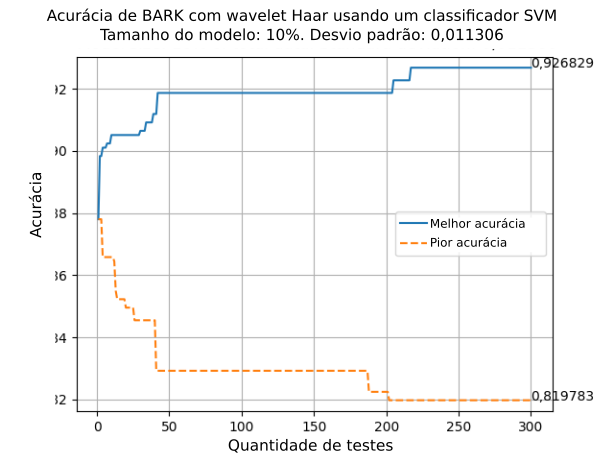
\includegraphics[width=\linewidth]{../monography/images/results/confusionMatrices/classifier_SVM_10}
				\caption{Acurácia \textit{X} quantidade de testes - SVM, modelo a 10\%}
			\end{figure}
			
			\column{0.5\textwidth}
			\begin{figure}
				\centering
				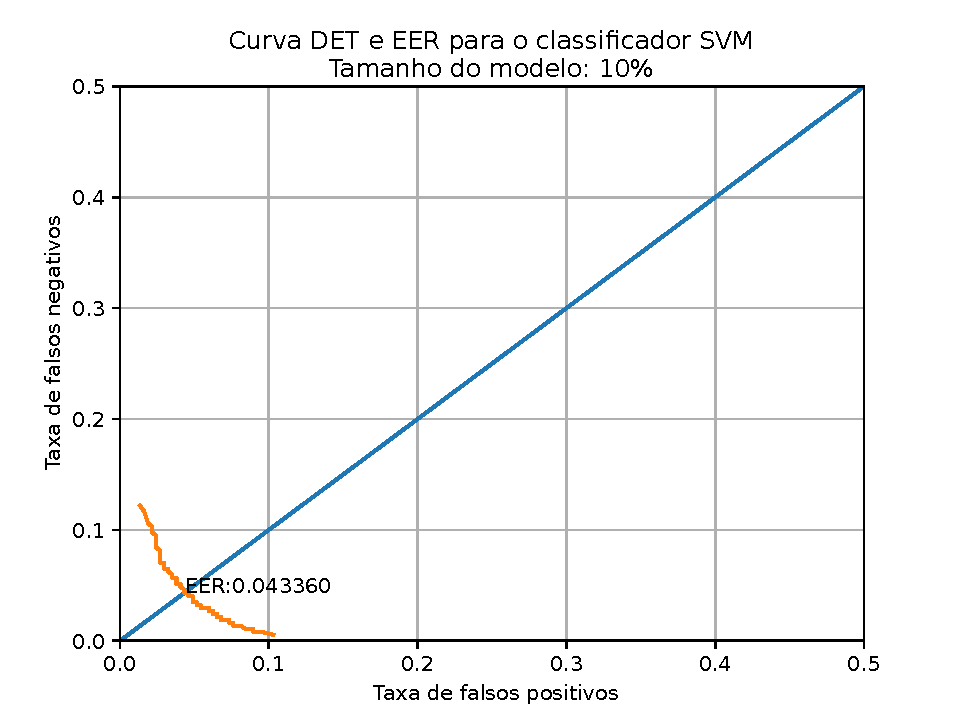
\includegraphics[width=\linewidth]{../monography/images/results/det/DET_for_classifier_SVM_10}
				\caption{Curva DET dos resultados de SVM, modelo a 10\%}
			\end{figure}
		\end{columns}
	}
	\only<2>{
		\begin{columns}
			\column{0.5\textwidth}
			\begin{figure}
				\centering
				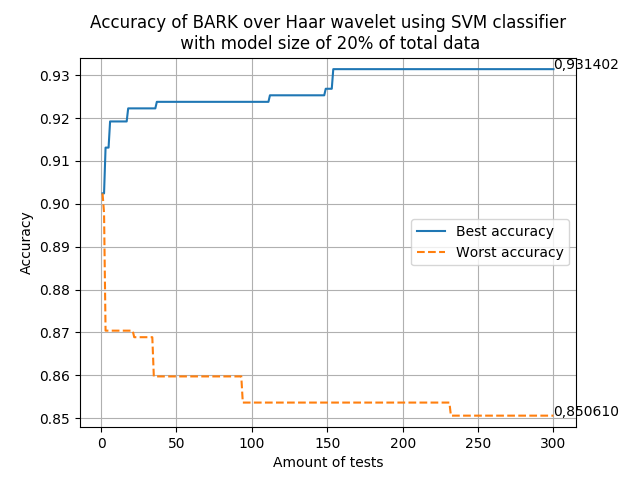
\includegraphics[width=\linewidth]{../monography/images/results/confusionMatrices/classifier_SVM_20}
				\caption{Acurácia \textit{X} quantidade de testes - SVM, modelo a 20\%}
			\end{figure}
			
			\column{0.5\textwidth}
			\begin{figure}
				\centering
				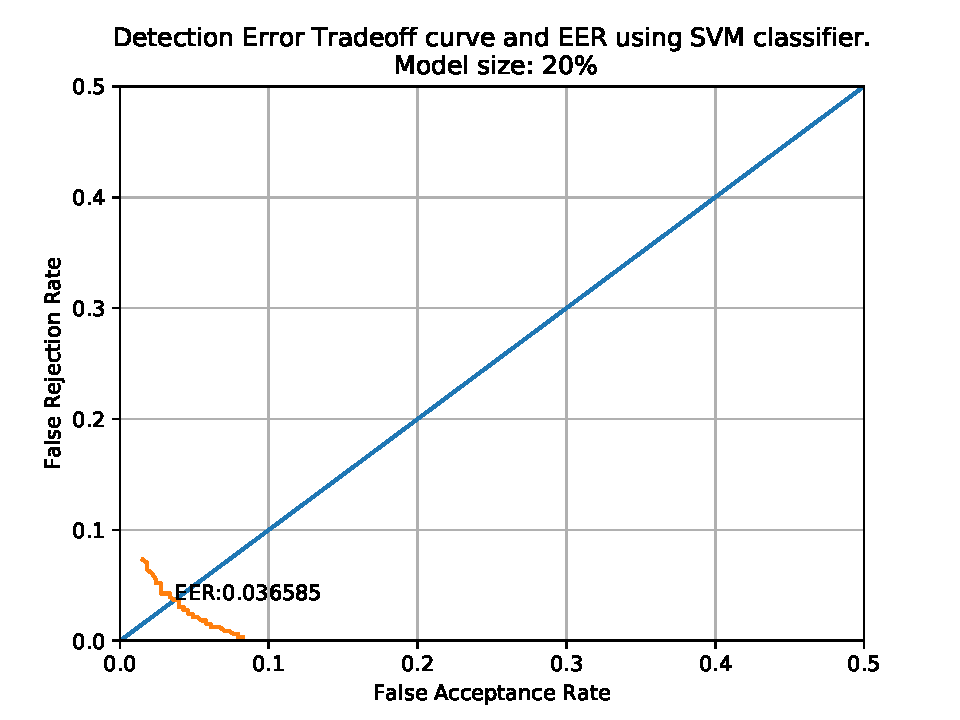
\includegraphics[width=\linewidth]{../monography/images/results/det/DET_for_classifier_SVM_20}
				\caption{Curva DET dos resultados de SVM, modelo a 20\%}
			\end{figure}
		\end{columns}
	}
	\only<3>{
		\begin{columns}
			\column{0.5\textwidth}
			\begin{figure}
				\centering
				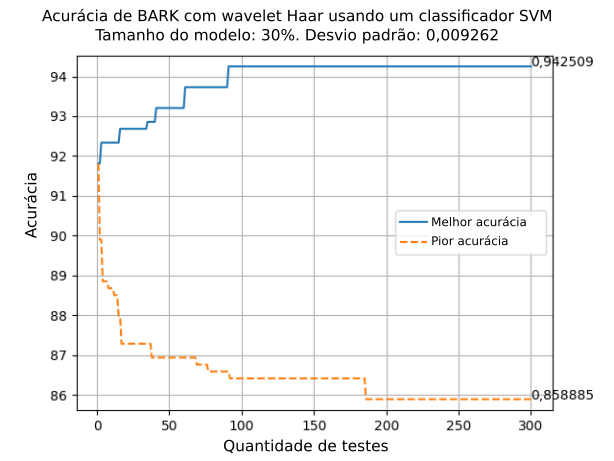
\includegraphics[width=\linewidth]{../monography/images/results/confusionMatrices/classifier_SVM_30}
				\caption{Acurácia \textit{X} quantidade de testes - SVM, modelo a 30\%}
			\end{figure}
			
			\column{0.5\textwidth}
			\begin{figure}
				\centering
				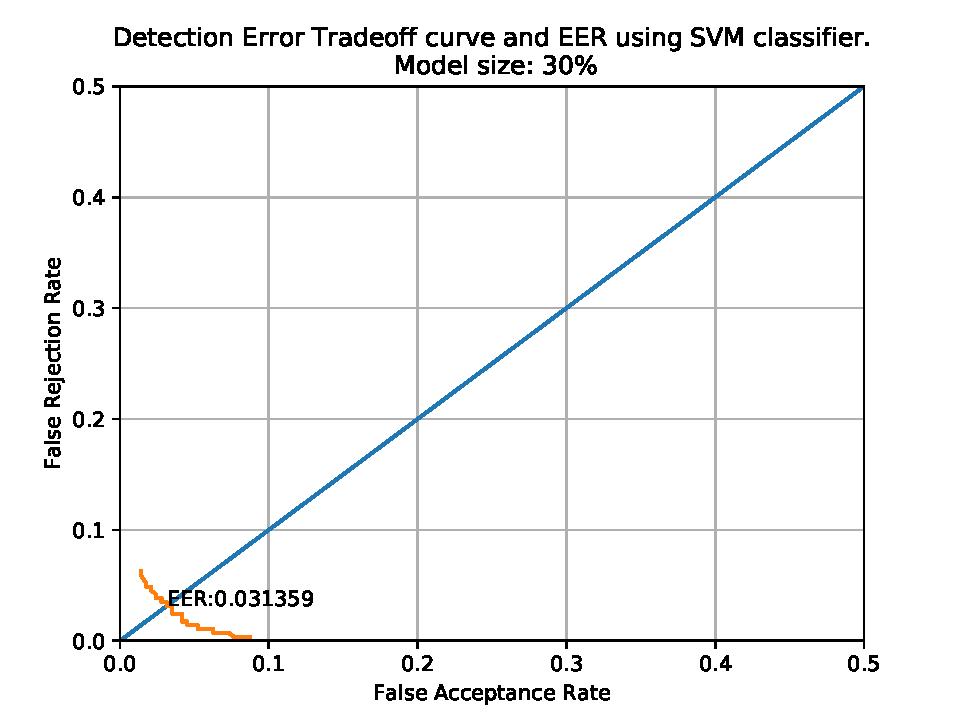
\includegraphics[width=\linewidth]{../monography/images/results/det/DET_for_classifier_SVM_30}
				\caption{Curva DET dos resultados de SVM, modelo a 30\%}
			\end{figure}
		\end{columns}
	}
	\only<4>{
		\begin{columns}
			\column{0.5\textwidth}
			\begin{figure}
				\centering
				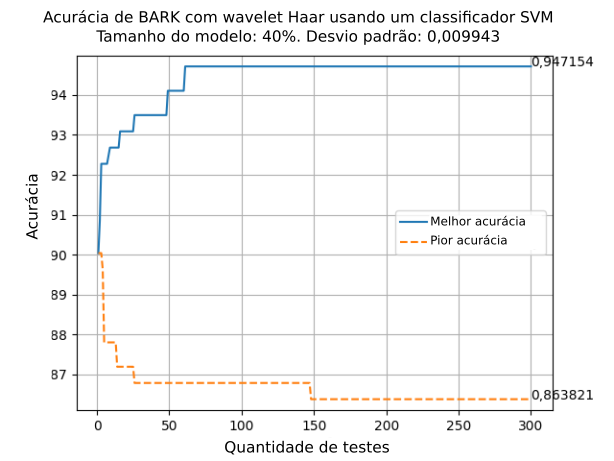
\includegraphics[width=\linewidth]{../monography/images/results/confusionMatrices/classifier_SVM_40}
				\caption{Acurácia \textit{X} quantidade de testes - SVM, modelo a 40\%}
			\end{figure}
			
			\column{0.5\textwidth}
			\begin{figure}
				\centering
				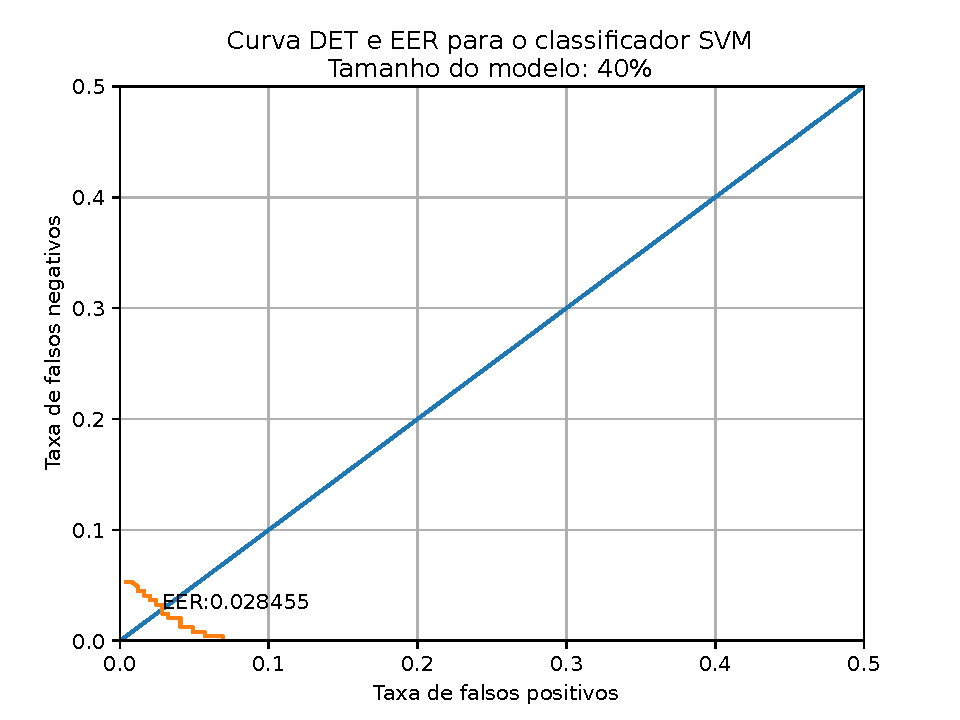
\includegraphics[width=\linewidth]{../monography/images/results/det/DET_for_classifier_SVM_40}
				\caption{Curva DET dos resultados de SVM, modelo a 40\%}
			\end{figure}
		\end{columns}
	}
	\only<5>{
		\begin{columns}
			\column{0.5\textwidth}
			\begin{figure}
				\centering
				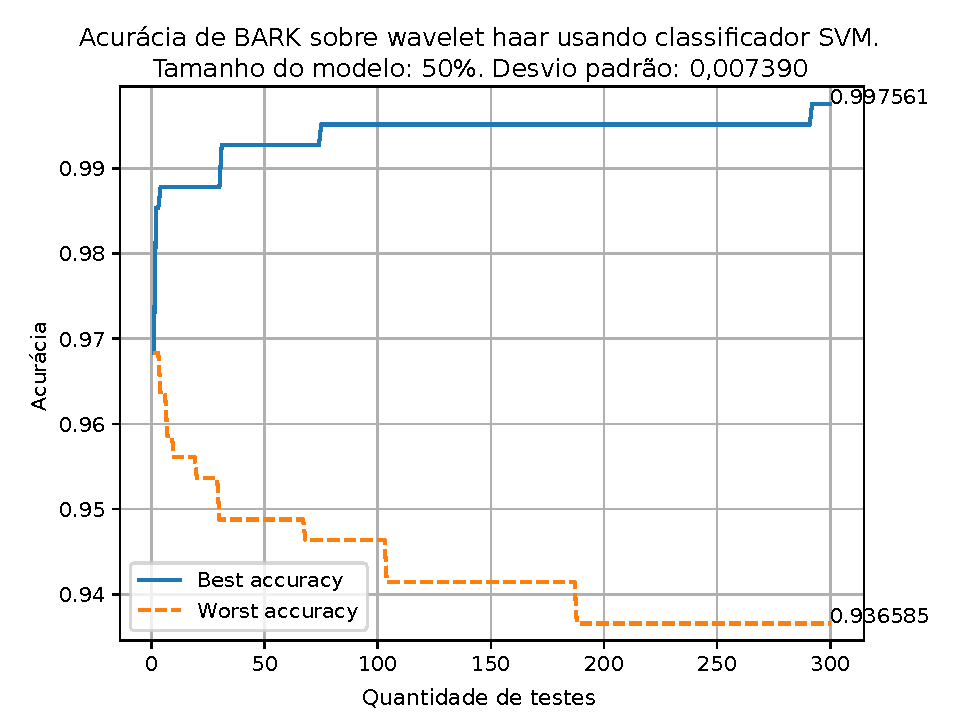
\includegraphics[width=\linewidth]{../monography/images/results/confusionMatrices/classifier_SVM_50}
				\caption{Acurácia \textit{X} quantidade de testes - SVM, modelo a 50\%}
			\end{figure}
			
			\column{0.5\textwidth}
			\begin{figure}
				\centering
				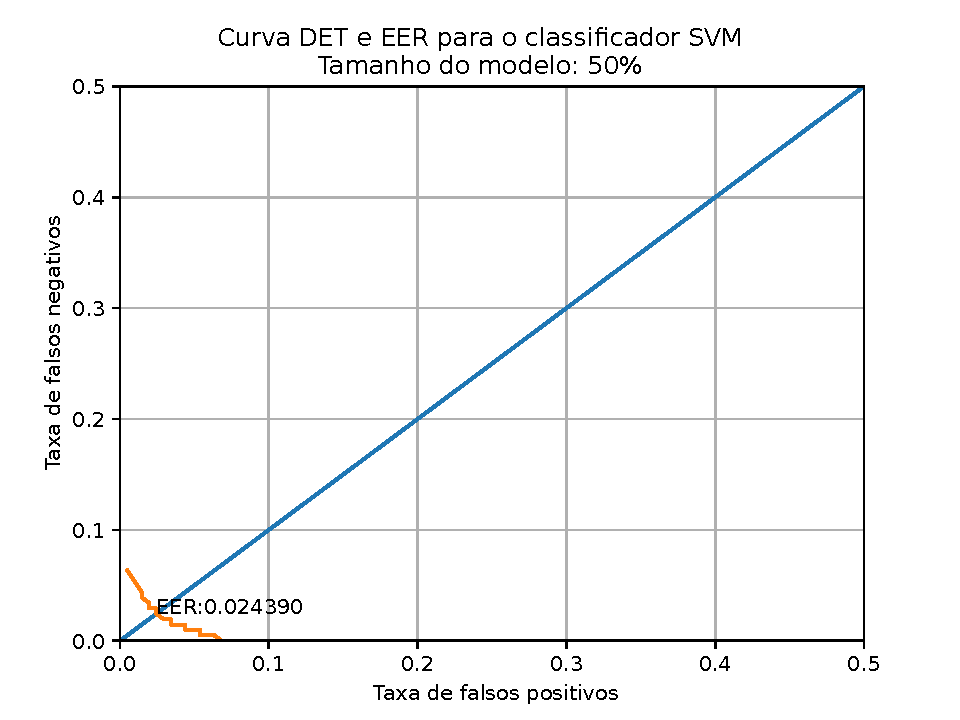
\includegraphics[width=\linewidth]{../monography/images/results/det/DET_for_classifier_SVM_50}
				\caption{Curva DET dos resultados de SVM, modelo a 50\%}
			\end{figure}
		\end{columns}
	}
\end{frame}

\begin{frame}
	\frametitle{Procedimento 03}
	\framesubtitle{Síntese}
	\par Dentre os testes realizados o melhores resultados foram:
	\begin{itemize}
		\item Acurácia: 0,997561.
		\item ERR: 0,02439.
	\end{itemize}
\end{frame}